\documentclass[12pt, a4paper]{article}

\usepackage[utf8]{inputenc}
\usepackage[T1]{fontenc}
\usepackage[russian]{babel}
\usepackage[oglav,spisok,boldsect, figwhole]{./style/fn2kursstyle}
\graphicspath{{./style/}{./figures/}}
\usepackage{float}%"Плавающие" картинки
\usepackage{multirow}
\usepackage{subcaption}
\usepackage{comment}
\usepackage{soul,color}
\usepackage{makecell}
\usepackage{amsfonts}
%Параметры титульника
\title{Математическое моделирование термоупругого разрушения хрупкого материала}
\group{ФН2-52Б}
\author{Г.А.~Швецов}
\supervisor{М.П.~Галанин}
\date{2023}
\begin{document}
	\newcommand{\pl}{\partial}
	\maketitle
	\tableofcontents
	
	
	\newpage
	\section-{Введение}
	При создании, проектировании и конструировании объектов для нашей жизни ставится задача об их надежности в различных условиях. Для этого требуются обширные знания из теории упругости. Анализ прочности конструкций и их разрушения являются проблемами, которые не теряют свою актуальность. 
		
	Основной интерес задач прочности представляет предугадывание различных вариантов разрушений, оценка прочности, влияние внешних факторов на процесс разрушения.
	
	Один из подразделов теории упругости --- \textit{теория термоупругости}. Неравномерное тепловое расширение в общем случае не может происходить свободно в сплошном теле, оно вызывает тепловые (температурные) напряжения. Знание величины и характера действия тепловых напряжений необходимо для всестороннего анализа прочности конструкции. Тепловые напряжения сами по себе и в сочетании с механическими напряжениями от внешних воздействий могут вызывать появление трещин и разрушение конструкции материала с повышенной хрупкостью. Согласно теории Дюамеля и Неймана, полная деформация является суммой упругой и тепловой деформаций.
	
		Цель настоящей работы --- построение и анализ одномерной модели разрушения стержня, обладающего физическими свойствами и характеристиками диоксида урана (UO$_2$), а также рассмотрение аналитического решения для линейного случая.
	
	
	
	
	\newpage
	\section{Постановка задачи}	

Термоупругость --- раздел механики твердого деформируемого тела, обобщающий теорию упругости для деформаций при неравномерном нагреве деформируемых тел. Общая задача математического моделирования термоупругости заключается в определении при заданных внешних механических и тепловых воздействиях тензора напряжений, тензора деформаций, вектора перемещения и скаляра температуры, удовлетворяющих уравнениям движения, уравнению теплопроводности, и соотношениям между напряжениями и деформациями и между деформациями и перемещениями.
	\subsection{Тензор малых деформаций Коши}
	Под действием внешних сил или в результате теплового воздействия твердое тело меняет свои размеры и форму, т.е. \textbf{деформируется}, при этом масса тела остается постоянной. Тензором деформации называют тензор, который характеризует сжатие (растяжение) и изменение формы в каждой точке тела при деформации.
	 Для математического описания деформации тела поступают следующим образом.
	
	Положение каждой точки тела $X_i(x_1,\dots,x_n)$ определяется ее радиус-вектором $\vec{r}=\vec{r}(X_i)$. Тогда вектор деформации, описывающий смещение точки тела определяется
	\begin{equation}
\vec u(u_1,\dots,u_n) = \vec r(X_i ')-\vec r(X_i)=\vec r'-\vec r,
	\end{equation}
	где $X_i$ и $X_i'$ --- вектора координат точек до и после деформации соответственно.
	
	
%	\begin{figure}[H]
%		\centering
%		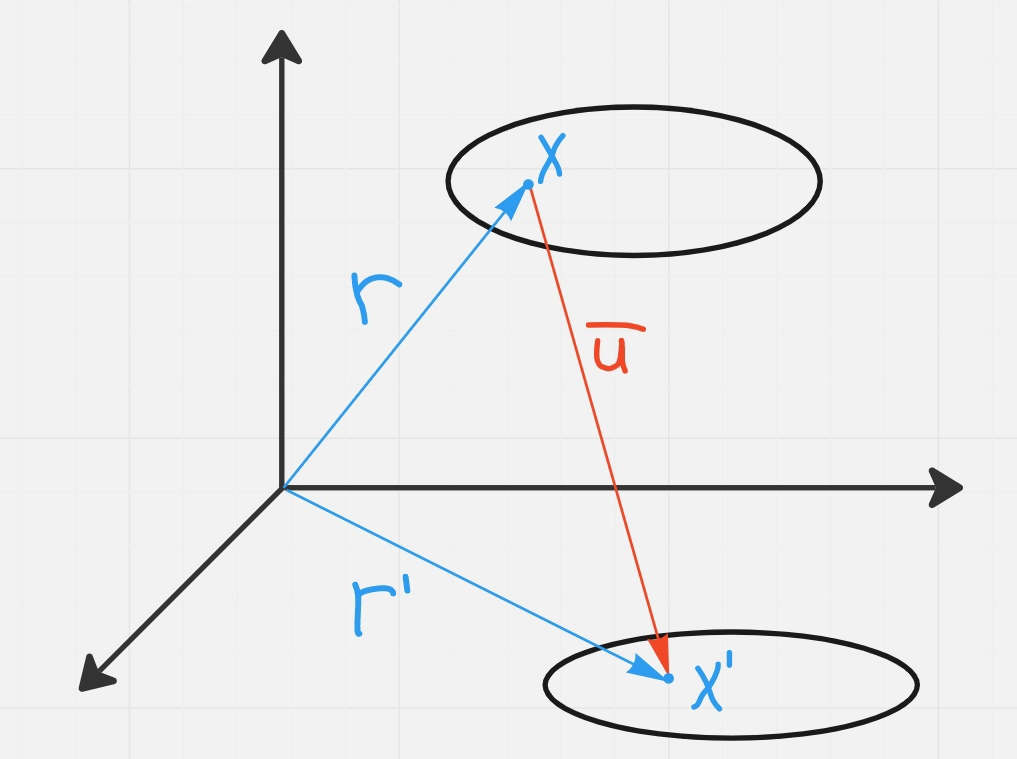
\includegraphics[width=0.8\linewidth]{p1}
%	\end{figure}
	При деформировании тела меняются расстояния между его точками. Рассмотрим две бесконечно близкие точки. Если радиус-вектор между ними до деформации задается величиной $dX$, то в деформированном теле радиус-вектор между теми же двумя точками определяется как
	\begin{equation}
dX'= dX+du = dx_k'=dx_k+du_k.
	\end{equation}
	Квадраты расстояний между заданными точками до и после приложения сил вычисляются по определению:
	\[
	(dl)^2=\sum_{k=1}^{n}(dx_k)^2,\quad
	(dl')^2=\sum_{k=1}^{n}(dx_k+du_k)^2.
	\]
	Используя определение полного дифференциала $du_k = \sum\limits_{l=1}^n\sfrac{\pl u_k}{\pl x_l}dx_l$ и правило суммирования по повторяющимся индексам, преобразуем величину $(dl')^2$ 
	\[
	(dl')^2=\sum_{k=1}^{n}\left(dx_k+\sum_{l=1}^n\sfrac{\pl u_k}{\pl x_l}dx_l\right)^2 =
	\sum_{k=1}^{n}\left((dx_k)^2+2\sfrac{\pl u_k}{\pl x_l}dx_l dx_k+\left(\sfrac{\pl u_k}{\pl x_l}dx_l\right)^2\right).
	\]
	Запишем в упрощенном виде
	\begin{equation}
(dl')^2 = (dl)^2+2\sfrac{\pl u_k}{\pl x_l}dx_l dx_k+\left(\sfrac{\pl u_k}{\pl x_l}dx_l\right)^2.
	\end{equation}

При малых деформациях третьим слагаемым можно пренебречь в силу его большего порядка малости. Во втором слагаемом индексы $k,\,l$ являются немыми, поэтому его можно записать в симметричном виде
	\begin{equation}
	\frac{\pl u_k}{\pl x_l}dx_ldx_k=\frac12\left(\frac{\pl u_k}{\pl x_l}+\frac{\pl u_l}{\pl x_k}\right)dx_ldx_k=\varepsilon_{kl}dx_ldx_k,
	\end{equation}
где $\varepsilon_{kl}$ --- составляющая тензора деформаций в точке $X$.

Симметричный тензор второго ранга $\hat\varepsilon$ с компонентами 
\begin{equation}
	\varepsilon_{kl}=\frac12\left(\frac{\pl u_k}{\pl x_l}+\frac{\pl u_l}{\pl x_k}\right), \quad k,\,l=1,2,3
	\label{eq:1.5}
\end{equation}
будем называть \textbf{тензором малой деформации.}

\textit{Соотношения Коши} (\ref{eq:1.5}) связывают три составляющие \textit{вектора перемещения} $\vec u$ с шестью (вследствие симметрии) компонентами тензора деформации $\hat\varepsilon$.

	
	
	 \subsection{Физический смысл компонент тензора деформаций}
	 Рассмотрим трехмерный случай. Матрица компонент тензора деформаций записывается в виде
	 \begin{equation}
	\varepsilon_{kl} = 
\begin{pmatrix}
	\varepsilon_{11}&\varepsilon_{12}&\varepsilon_{13}\\
	\varepsilon_{21}&\varepsilon_{22}&\varepsilon_{23}\\
	\varepsilon_{31}&\varepsilon_{32}&\varepsilon_{33}
\end{pmatrix}
=
\begin{pmatrix}
	\varepsilon_x&\frac12\gamma_{xy}&\frac12\gamma_{xz}\\
	\frac12\gamma_{yx}&\varepsilon_y&\frac12\gamma_{yz}\\
	\frac12\gamma_{zx}&\frac12\gamma_{zy}&\varepsilon_z
\end{pmatrix}.
	 \end{equation}
% \begin{figure}[H]
%	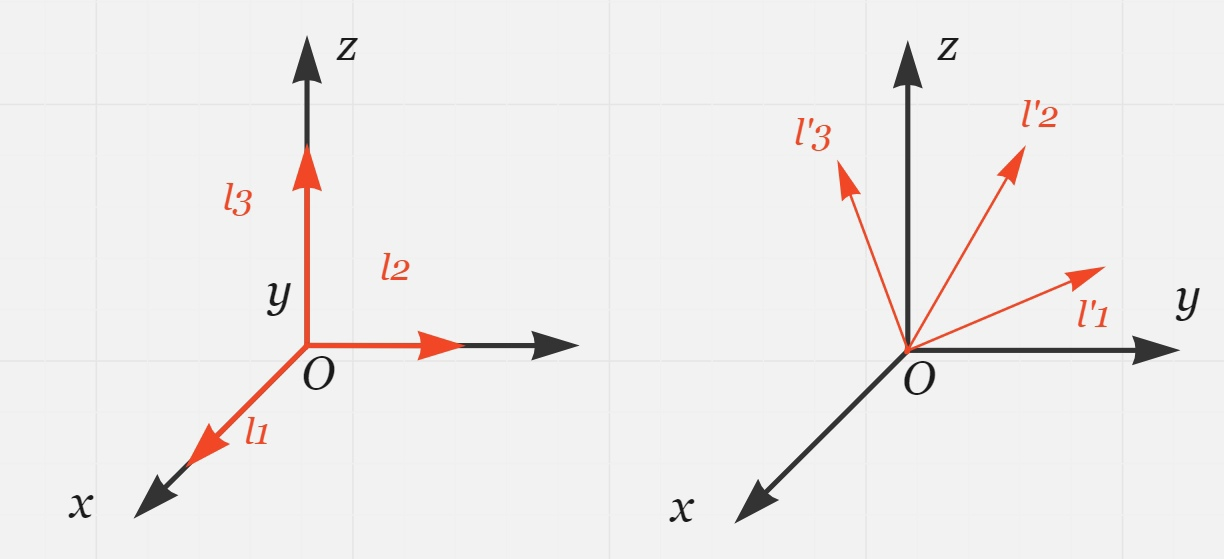
\includegraphics[width=\textwidth]{p2}
% \end{figure}
  Диагональные элементы $\varepsilon_x,\,\varepsilon_y,\,\varepsilon_z$ --- это коэффициенты относительного удлинения отрезков, которые до деформации были параллельны осям $x,\,y,\,z.$
  \[
  \varepsilon_x = \frac{l'_1-l_1}{l_1} = \frac{\Delta l'_1}{l_1},\quad \varepsilon_y = \frac{l'_2-l_2}{l_2} = \frac{\Delta l'_2}{l_2},\quad \varepsilon_z = \frac{l'_3-l_3}{l_3} = \frac{\Delta l'_3}{l_3},\quad
  \]
\begin{figure}[H]
	\centering
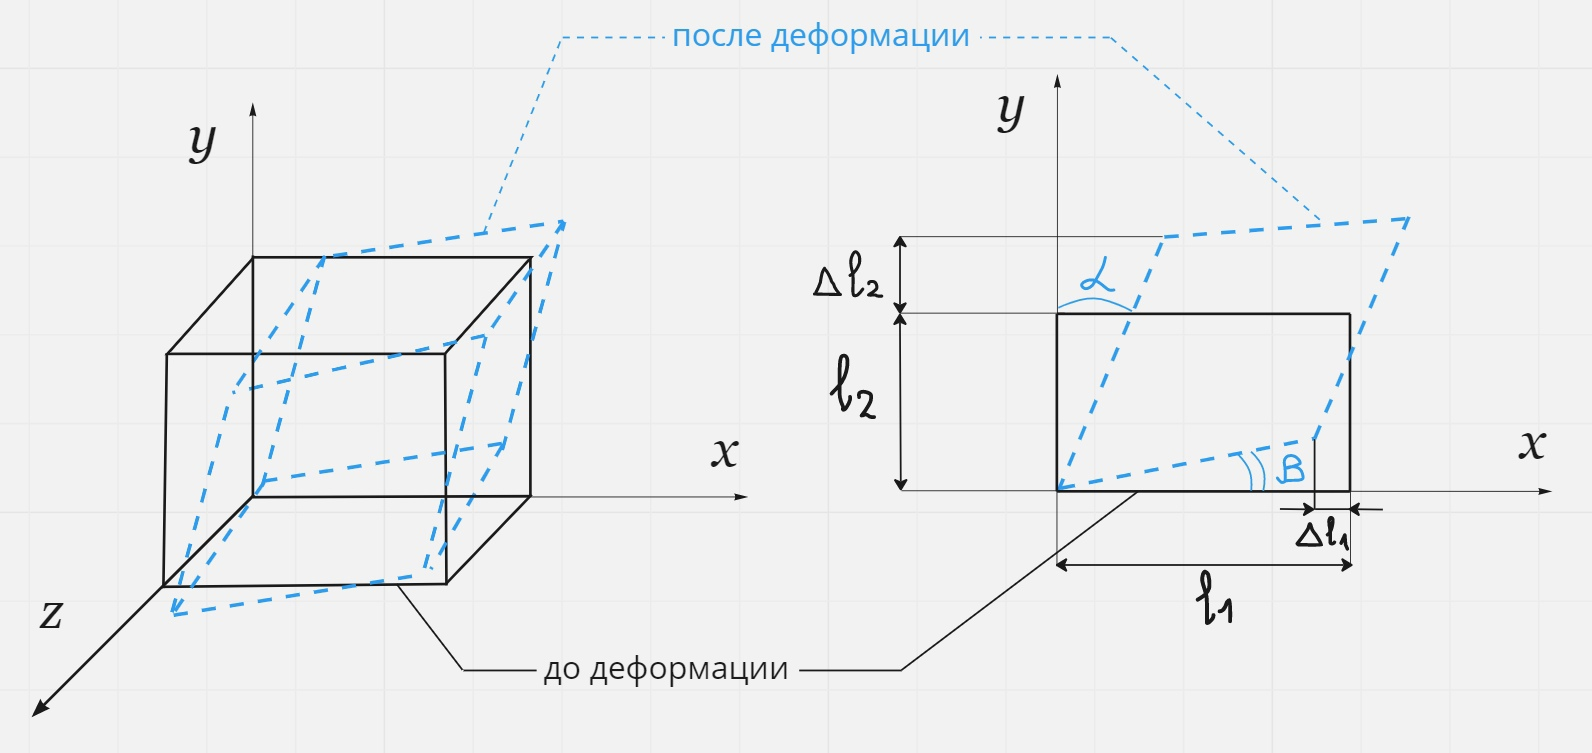
\includegraphics[width=0.82\textwidth]{p3}
\caption{Физический смысл}
\label{fig:p3}
\end{figure}
  Внедиагональные элементы $\varepsilon_{kl},\,k \ne l$ определяют угол сдвига или угловую деформацию. В частности, для плоскости $xy$ (см. рис.~\ref{fig:p3}) $\gamma_{xy} = \alpha+\beta$.
  
		
	\subsection{Внешние силы и тензор напряжений}
Существуют два вида внешних сил, которые могут воздействовать на тело. Силы, распределенные по поверхности тела, такие, как давление одного тела на другое, называются \textbf{поверхностными силами}. Силы, распределенные по массе тела, такие, как силы тяжести, силы инерции, называются \textbf{массовыми силами} (объемные силы).

\textbf{Плотность объемных сил} характеризует вектор
\begin{equation}
	\boldsymbol b(M) = \lim\limits_{d\to0}\frac{\Delta \boldsymbol F}{\Delta V},
\end{equation}
где $\Delta \boldsymbol F$ --- вектор силы, распределенной в объеме $\Delta V$ среды в окрестности точки $M$.

\textbf{Плотность поверхностных сил} характеризует вектор
\begin{equation}
	\boldsymbol p(N) = \lim\limits_{d\to0}\frac{\Delta \boldsymbol P}{\Delta S},
\end{equation}
где $\Delta \boldsymbol P$ --- вектор силы, действующий на элементарную площадку $\Delta S$ поверхности $S$, ограничивающей тело объемом $V$ \cite{zarubin}.
	
Механическое напряжение есть мера внутренних сил, возникающих в деформированном теле под действием внешних сил.
	
	Рассмотрим случай, когда напряжения во всем теле однородны и все части тела находятся в состоянии статического равновесия. Выделим в таком теле единичный куб с ребрами, параллельными осям координат $x,\,y,\,z$.
	\begin{figure}[H]
		\centering
		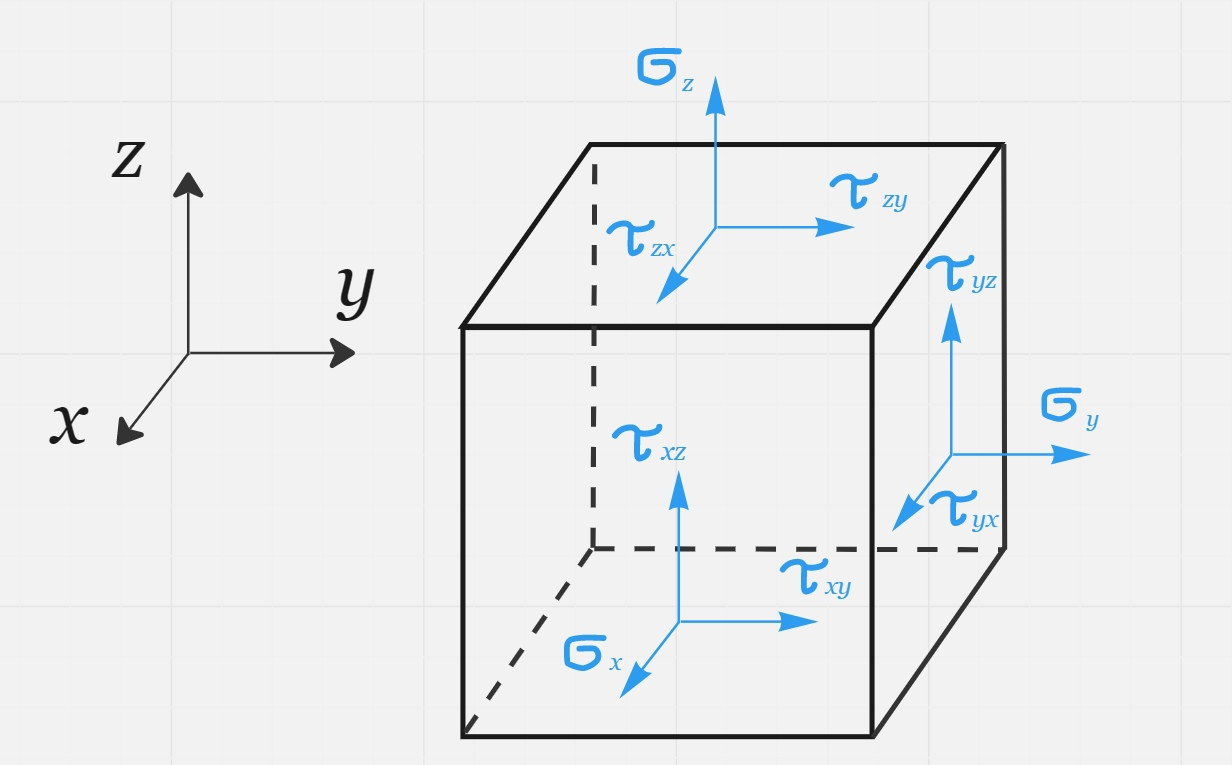
\includegraphics[width=12cm]{p6}
		\caption{Элементарный объем тела --- куб}
		\label{fig:p6}
	\end{figure}
Силы, действующие на противоположные грани куба в условиях равновесия, одинаковы, поэтому достаточно рассмотреть только те, которые действуют на непараллельные грани. Чтобы обозначить напряжения, действующие на шести гранях куба, потребуется три символа $\sigma_x,\,\sigma_y,\,\sigma_z$ для нормальных напряжений и шесть $\tau_{xy},\,\tau_{yx},\,\tau_{yz},\\\tau_{zy},\,\tau_{xz},\,\tau_{zx}$ для касательных (см. рисунок~\ref{fig:p6}).

Согласно закону парности касательных напряжений на двух площадках, проходящих через данную точку, выполняются следующие равенства
\[
\tau_{xy} = \tau_{yx};\quad \tau_{yz} = \tau_{zy};\quad \tau_{xz} = \tau_{zx}.
\]
Из приведенных равенств вытекает, что независимыми являются только 6 компонент напряжений.

Таким образом, для описания напряженного состояния в точке вводится \textbf{тензор напряжений} $\boldsymbol{\hat\sigma}$ ---  симметричный тензор второго ранга, описывающий механические напряжения в произвольной точке нагруженного тела, возникающих в этой точке при его малых деформациях.
\begin{equation}
\sigma_{ij} = 
\begin{pmatrix}
	\sigma_{11}&\sigma_{12}&\sigma_{13}\\
	\sigma_{21}&\sigma_{22}&\sigma_{23}\\
	\sigma_{31}&\sigma_{32}&\sigma_{33}
\end{pmatrix} =
\begin{pmatrix}
	\sigma_{11}&\tau_{12}&\tau_{13}\\
	\tau_{21}&\sigma_{22}&\tau_{23}\\
	\tau_{31}&\tau_{32}&\sigma_{33}
\end{pmatrix},
\end{equation}
где $\sigma_{ii}$ --- нормальные напряжения, $\tau_{ij}$ --- касательные напряжения \cite{kovalenko}.

Если рассматривать окрестность точки $N$ поверхности $S$ с единичным вектором $\boldsymbol n(N)$ внешней нормали при заданном векторе $\boldsymbol p(N)$ плотности поверхностных сил с проекциями $p_i(N)$ на оси пространственных координат:
\begin{equation}
	\boldsymbol{\hat \sigma} \cdot \boldsymbol n(N) = \boldsymbol p(N),\quad\text{ или }\quad \sigma_{ji}(N)n_j(N)=p_i(N),\; N \in S. 
	\label{eq:1.10}
\end{equation}

\subsection{Температурные деформации и напряжения}
В предположении существования аддитивного разложения компонент тензора малых деформаций Коши запишем
\begin{equation}
	\varepsilon_{kl} = \frac12\left(\frac{\pl u_k}{\pl x_l}+\frac{\pl u_l}{\pl x_k}\right)=\varepsilon_{kl}^e+\varepsilon_{kl}^0=\varepsilon_{kl}^e+\varepsilon_{kl}^T,\quad k,\,l=1,2,3,
	\label{eq:1.11}
\end{equation}
где $\varepsilon_{ij}^e$ --- компоненты упругой составляющей тензора деформаций, а $\varepsilon_{ij}^0$ --- компоненты тензора неупругих деформаций (в нашем случае температурные деформации).	

Пусть  тело в исходном недеформированном состоянии имеет температуру $T_0=\mathrm{const}$. Для большинства конструкционных материалов температурная деформация $\varepsilon_{kl}^T$ является пропорциональной изменению температуры $\Delta T$, т.е. 
\[
\hat{\varepsilon}^T = \alpha \Delta T = \alpha(T-T_0),
\]
где $\alpha$ --- коэффициент температурного расширения, $\Delta T = T(\mathbf{x},t) - T_0$ --- приращение температуры относительно уровня нулевых деформаций. Согласно принятому в мире <<знаковому соглашению>> температурное расширение считается положительным, а температурное сокращение --- отрицательным \cite{kovalenko}.

	\subsection{Обобщенный закон Гука}	
	В общем случае напряжения и деформации описываются тензорами второго ранга в трехмерном пространстве (имеют по 9 компонент). Связывающий их \textit{тензор коэффициентов упругости} является тензором четвертого ранга $C_{ijkl}$ и содержит 81 коэффициент. Его вид определяется моделью рассматриваемой среды.
	
	Данный тензор является материальной константой упругости \textit{анизотропных}\footnote{Анизотропия --- различие свойств среды в различных направлениях внутри этой среды.} материалов. Вследствие симметрии тензоров напряжений $\sigma_{ij}$ и деформаций $\varepsilon_{kl}$, а также симметрии тензора $C_{ijkl}$ по первой паре индексов, второй паре индексов и по парам индексов ($C_{ijkl},\, C_{jikl},\,C_{ijlk},\,C_{klij}$), независимыми являются только 21 постоянная \cite{timoshenko}.
	
	\textbf{Закон Гука} выглядит следующим образом
	\begin{equation}
			\sigma_{ij} = C_{ijkl} \varepsilon_{kl}^e, \qquad i,\,j,\,k,\,l = 1,2,3.
			\label{Hook}
	\end{equation}
	
	Согласно \textit{нотации Фойгта}\footnote{\textbf{Нотация Фойгта} --- матричная форма записи симметричного тензора 4-го ранга. Впервые была предложена немецким физиком Вольдемаром Фойгтом для тензора упругости в формулировке закона Гука для анизотропных материалов.} тензору коэффициентов упругости можно поставить в соответствие матрицу $\hat{C}$ вида:
	 \[
	\hat{C} = 
	\begin{pmatrix}
		C_{11} & C_{12} & C_{13} & 0 & 0 & 0 \\
		C_{21} & C_{22} & C_{23} & 0 & 0 & 0 \\
		C_{31} & C_{32} & C_{33} & 0 & 0 & 0 \\
		0 &      0 &      0 & C_{44} & 0 & 0 \\
		0 &      0 &      0 & 0 & C_{55} & 0 \\
		0 &      0 &      0 & 0 & 0 & C_{66} \\
	\end{pmatrix} 
	=
	\begin{pmatrix}
		C_{11} & C_{12} & C_{12} & 0 & 0 & 0 \\
		C_{12} & C_{11} & C_{12} & 0 & 0 & 0 \\
		C_{12} & C_{12} & C_{11} & 0 & 0 & 0 \\
		0 &      0 &      0 & C_{44} & 0 & 0 \\
		0 &      0 &      0 & 0 & C_{44} & 0 \\
		0 &      0 &      0 & 0 & 0 & C_{44} \\
	\end{pmatrix} 
	\] 
	
	Тензор упругости для \textit{изотропного}\footnote{Изотропия --- неизменность свойств среды во всех направлениях.} материала: упругие свойства определяются двумя константами (постоянными Ламэ $\lambda \text{ и } \mu$):
	\begin{gather*}
	C_{44}=C_{55}=C_{66}=\frac12(C_{11}-C_{12}),\\
	C_{11} =\lambda+2\mu,\;C_{12} = \lambda,\; C_{44} = \mu.
	\end{gather*}
	Тогда матрица $\hat{C}$ выглядит следующим образом:
	\begin{equation}
		\hat{C} = 
		\begin{pmatrix}
			\lambda + 2\mu & \lambda & \lambda & 0 & 0 & 0 \\
			\lambda & \lambda + 2\mu & \lambda & 0 & 0 & 0 \\
			\lambda & \lambda & \lambda + 2\mu & 0 & 0 & 0 \\
			0 &      0 &      0 & \mu & 0 & 0 \\
			0 &      0 &      0 & 0 & \mu & 0 \\
			0 &      0 &      0 & 0 & 0 & \mu \\
		\end{pmatrix} 
		\label{Flex}
	\end{equation}

	Возвращаясь к выражению (\ref{Hook}) и подставив туда матрицу (\ref{Flex}), мы получаем
	\[
	\begin{pmatrix}
		\sigma_{11} \\
		\sigma_{22} \\
		\sigma_{33} \\
		\sigma_{23} \\
		\sigma_{13} \\
		\sigma_{12} \\
	\end{pmatrix}
	= 
	\begin{pmatrix}
		\lambda + 2\mu & \lambda & \lambda & 0 & 0 & 0 \\
		\lambda & \lambda + 2\mu & \lambda & 0 & 0 & 0 \\
		\lambda & \lambda & \lambda + 2\mu & 0 & 0 & 0 \\
		0 &      0 &      0 & \mu & 0 & 0 \\
		0 &      0 &      0 & 0 & \mu & 0 \\
		0 &      0 &      0 & 0 & 0 & \mu \\
	\end{pmatrix} 
	\begin{pmatrix}
		\varepsilon_{11} \\
		\varepsilon_{22} \\
		\varepsilon_{33} \\
		2\varepsilon_{23} \\
		2\varepsilon_{13} \\
		2\varepsilon_{12} \\
	\end{pmatrix}
	\]	
	\noindent или в матричной форме
	\[
	\begin{split}
		\begin{bmatrix}
			\sigma_{11} & \sigma_{12} & \sigma_{13} \\
			\sigma_{21} & \sigma_{22} & \sigma_{23} \\
			\sigma_{31} & \sigma_{32} & \sigma_{33} \\
		\end{bmatrix}
		&= \,\,
		2\mu \begin{bmatrix}
			\varepsilon_{11} & \varepsilon_{12} & \varepsilon_{13} \\
			\varepsilon_{21} & \varepsilon_{22} & \varepsilon_{23} \\
			\varepsilon_{31} & \varepsilon_{32} & \varepsilon_{33} \\
		\end{bmatrix}
		+ \lambda \begin{bmatrix}
			\varepsilon_{11} & 0 & 0 \\
			0 & \varepsilon_{22} & 0 \\ 
			0 & 0 & \varepsilon_{33} 
		\end{bmatrix}
	\end{split}
	\]
	
	\subsection{Уравнения равновесия и граничные условия}
Обобщая \textit{закон сохранения количества движения материальной системы} на случай сплошной среды можно записать
\begin{equation}
	\frac{d\boldsymbol{Q}_v}{dt} = \int\limits_V \rho \frac{d\boldsymbol v}{dt}\,dV=\int\limits_S \boldsymbol p\,dS +\int\limits_V \boldsymbol b\,dV.
	\label{eq:1.9}
\end{equation}
Левая часть (\ref{eq:1.9}) соответствует скорости изменения во времени $t$ вектора количества движения $\boldsymbol{Q}_v$ среды, занимающей в \textit{актуальной конфигурации} область объемом $V$, ограниченным поверхностью $S$ ($\rho$ и $\boldsymbol v$ --- плотность среды и вектор скорости ее частиц соответственно). Правая часть (\ref{eq:1.9}) равна \textit{главному вектору системы сил}, характеризуемых в данном случае векторами $\boldsymbol p$ и $\boldsymbol b$ \textit{плотности поверхностных} и \textit{объемных сил} соответственно \cite{zarubin}.

Согласно соотношениям (\ref{eq:1.10}) и (\ref{eq:1.9}), с учетом \textit{теоремы Остроградского --- Гаусса} получим
\begin{equation}
	\rho \frac{dv_i}{dt} = \frac{\pl \sigma_{ji}}{\pl x_j}+b_i.
	\label{eq:1.14}
\end{equation}
В нашем случае неподвижной среды ($\boldsymbol v \equiv 0$) из (\ref{eq:1.14}) следует ее уравнения равновесия.
\begin{equation}
Ox_j:\;\frac{\pl \sigma_{ji}}{\pl x_j}+b_i = 0,\quad i = 1,\,2,\,3.
\end{equation}

Если тело закреплено, то любые перемещения его точек происходят за счет деформации, поэтому необходимо задать \textit{граничные условия}. В классической задаче теории упругости такие условия разделяют на два типа: \textit{кинематические} и \textit{силовые}. Предполагается, что каждый их них задан на своей части поверхности:
\[
\begin{split}
	S_u\colon& u_i(\vec x, t) = \widetilde{u_i}(\vec x, t), \\
	S_p\colon& \sigma_{ij}(\vec x) n_j(\vec x)  = \widetilde{p_i}(\vec x),  \\
\end{split}
\]

\noindent где $S = S_u \cup S_p$ --- поверхность рассматриваемого тела; $S_u$ --- часть поверхности, на которой заданы кинематические условия, $S_p$ --- силовые.


\subsection{Моделирование разрушения. Модель размазанных трещин.}

В основе модели размазанных трещин лежит изменение свойств материала, она применима только для тех тел, в которых образование микротрещин, пластическая деформация, разрывы деформаций и напряжений пренебрежимо малы. Например, керамика и бетон обладают этими свойствами \cite{smeared crack}.

При нагрузке хрупкого материала, процесс разрушения может быть описан, как разгрузка по всему объему в сочетании с дополнительным растяжением. На рис. \ref{fig:ceramic} видно, что пока напряжение меньше предела прочности $\sigma < \sigma_f$  и деформации меньше соответствующего значения $\varepsilon < \varepsilon_f$, материал ведет себя, как линейно-упругий, а затем происходит разгрузка по нелинейному закону.
\begin{figure}[h]
	\centering
	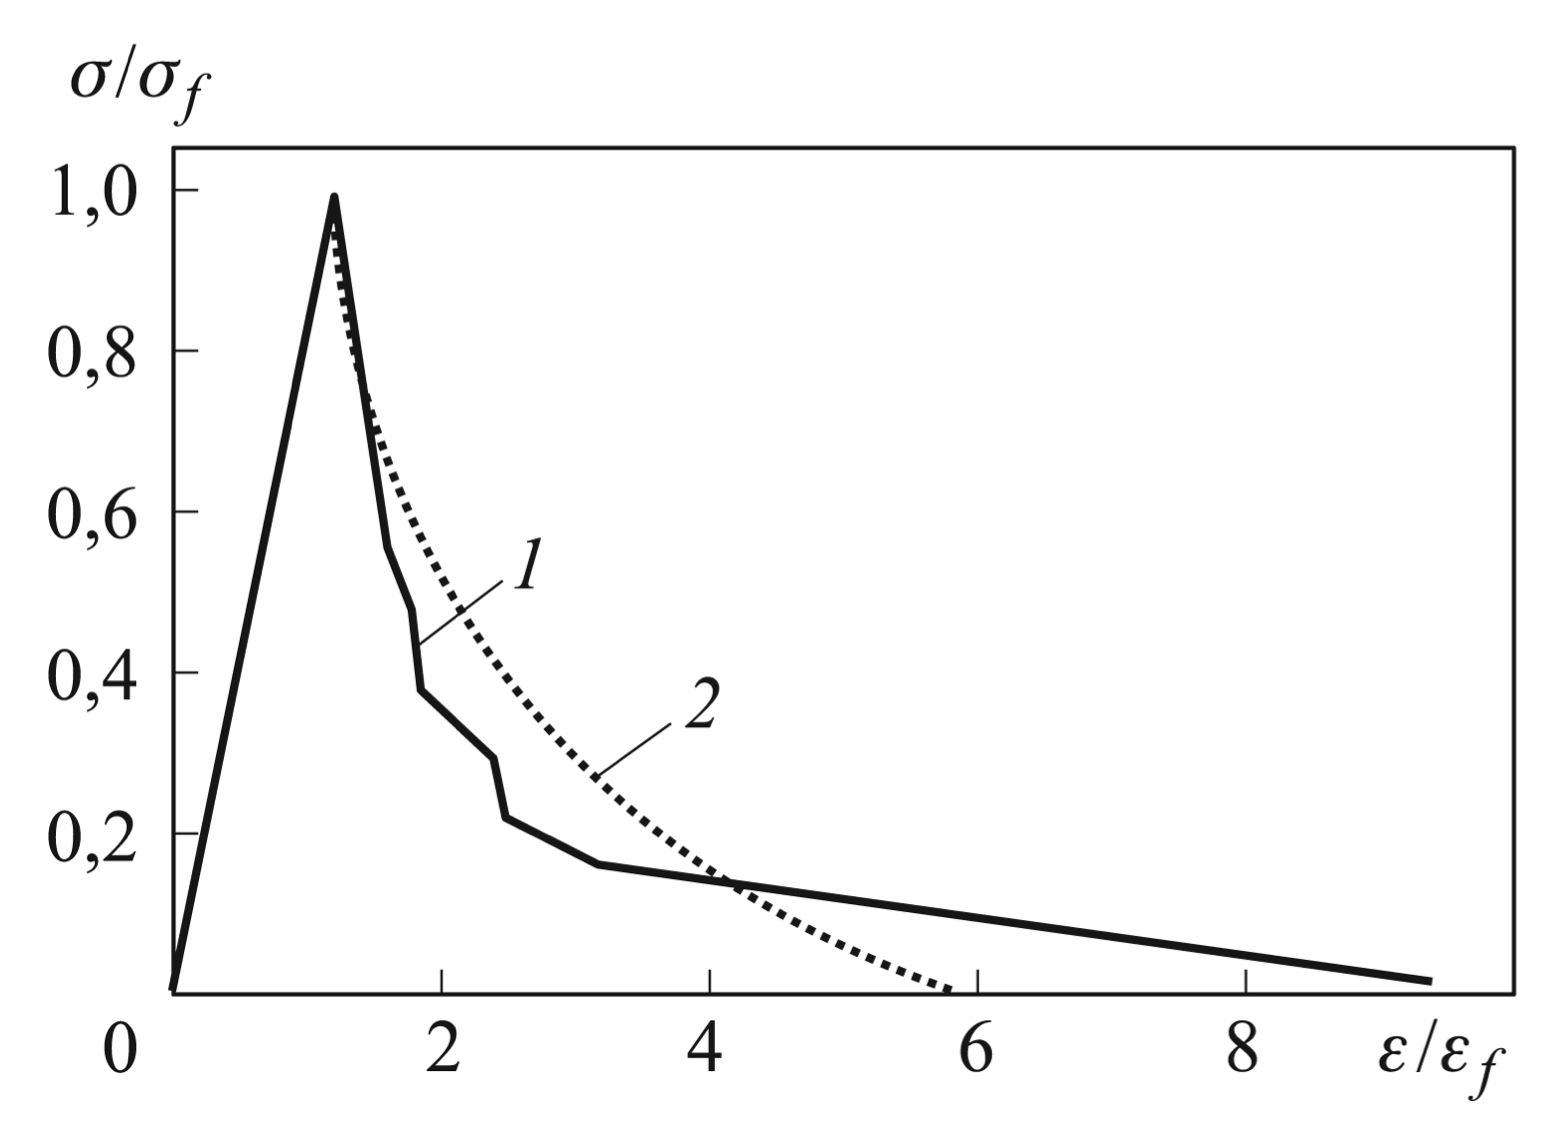
\includegraphics[width=0.55\textwidth]{ceramic}
	\caption{Экспериментальная (1) и аналитическая (2) кривые нормализованного растягивающего отклика для керамических материалов}
	\label{fig:ceramic}
\end{figure}

\pagebreak

При достижении предельного значения прочности $\sigma_f$ происходит инициализация трещины. Она формируется лишь после достижения значений деформаций, превышающих $\varepsilon_f$ в $5-10$ раз. Кривую, имеющую данный характер поведения, можно аппроксимировать в следующем виде:
\[
\dfrac{\sigma}{\sigma_f} = A + B e^{-C\tfrac{\varepsilon}{\varepsilon_f}},
\]

\noindent где $A \approx -0.024, B \approx 1.69, C \approx 0.5$.

Важно отметить, что модель размазанных трещин чувствительна к шагу сетки, что является ее главным недостатком \cite{galanin2}.


	\section{Одномерный случай}
	Рассмотрим одномерный стержень длины $l$, закрепленный на концах, а также квазистационарную задачу для него. Параметр $t$ --- возрастающий, он в данном случае имеет смысл времени. Для квазистационарной задачи будем решать уравнение равновесия на каждом временном слое: используем метод конечных разностей на равномерной сетке.
	
	Нелинейная модель упругости и образования трещин для зависимости напряжения от деформации выглядит следующим образом
	\begin{equation}
		\sigma(\varepsilon) =
		\begin{cases}
			E\varepsilon^e,& E\varepsilon^e<\sigma_f^v(\varepsilon),
			\\
			\sigma_f^v(\varepsilon),\,\sigma_f^v(\varepsilon)=\Biggl(A+Be^{-C\sfrac{\varepsilon-\varepsilon^T}{\varepsilon_f}}\Biggr),& E\varepsilon^e\ge\sigma_f^v(\varepsilon),
		\end{cases}
	\label{eq:2.1}
	\end{equation}
где $\varepsilon^e$ --- упругая деформация, $\sigma_f^v(\varepsilon)$ --- это переменный предел прочности, который в недеформированном состоянии материала равен пределу прочности $\sigma_f^v(0) = \sigma_f$, $E$ --- модуль Юнга.

Согласно аддитивному разложению (\ref{eq:1.11}) упругая составляющая деформаций определяется следующим выражением
\begin{equation}
\varepsilon^e = \varepsilon - \varepsilon^T-\varepsilon^{crk},	
\end{equation}
где $\varepsilon$ --- полная деформация, $\varepsilon^T$ --- температурная деформация, $\varepsilon^{crk}$ --- деформация за счет трещин (в линейном случае $\varepsilon^{crk}=0$), которая вычисляется по данным о текущем состоянии на данный момент:
\[
\varepsilon^{crk} = \varepsilon-\varepsilon^T-\frac{\sigma(\varepsilon)}{E}
\]

Будем прикладывать знакопеременную нагрузку по закону:
\[
T(x,t) = \tilde T+F(x)\tau(t),
\]
где $\tilde T$ --- усредненная по времени температура, $F(x)$ --- функция, описывающая пространственное распределение температуры, $\tau(t)$ --- функция времени.

Математическая модель для однородного стержня
\begin{equation}
	\begin{cases}
		T(x,t) = \tilde T+F(x)\tau(t),& t \ge 0,\; 0 \le x\le l;\\
		\sfrac{\pl \sigma}{\pl x} = 0,& 0<x<l;\\
		\sigma = \sigma(\varepsilon-\varepsilon^0);\\
		\varepsilon = \sfrac{\pl u}{\pl x};\\
		\varepsilon^T = \alpha(T-T_0);\\
		u(0,t) = u(l,t) = 0,		
	\end{cases}
\end{equation}
где $u$ --- перемещения, $T_0$ --- справочная температура, $\varepsilon^0 = \varepsilon^T$ --- температурная деформация. 

\section{Результаты вычислений}
Физические характеристики диоксида урана UO$_2$: 
\begin{itemize}
\item предел прочности $\sigma_f = 1,1\cdot 10^8$ Па;
\item предел деформации $\varepsilon_f=0.000628571$;
\item модуль Юнга $E = 1,75\cdot 10^{11}$ Па;
\item коэффициент теплового расширения $\alpha = 10^{-5}\text{ K}^{-1}$;
\item температура естественного состояния $T_0 = 300$ К.
\end{itemize}
Для упругого, линейного случая (\ref{eq:2.1}) составим дифференциальное уравнение:
\begin{gather*}
	\sigma(\varepsilon) = E\varepsilon^e=E(\varepsilon-\varepsilon^T)=E\left(\frac{\pl u}{\pl x}-\alpha(T(x,t)-T_0)\right),\\
\frac{\pl \sigma}{\pl x} = 0 \quad \Leftrightarrow \quad \frac{\pl^2u}{\pl x^2} = \alpha \frac{\pl T(\mathrm x,t)}{\pl x}.
\end{gather*}

Будем выбирать функцию $F(x)$ так, чтобы она была симметрична относительно середины стержня, например, $F(x) = \sin(\frac{\pi x}{l})$. Будем решать задачу методом конечных разностей на равномерной сетке. При значениях напряжений, которые больше предела прочности $\sigma_f$, материал разгружается по нелинейному закону, поэтому появляется необходимость решать нелинейное уравнение. Линеаризуем его, используя метод Ньютона.

Пусть $l = 10$ м, $T_f$ --- длительность измерения, $\tau_h = 0.005$ c --- временной шаг, $n = 10$ --- количество узлов сетки.
%Рассмотрим поведение стержня на четырех периодах нагружения. Поведение стержня будем рассматривать в точке $x=h$, где $h$ --- шаг сетки.
\begin{enumerate}
	\item Пусть $\quad F(x) = a \sin\left(\sfrac{\pi x}{l}\right),\quad \tau(t) = (t+1)\cos(\pi t^2),\quad a = 50,\quad T_f = 4 \text{ c}.$
	
	Аналитическое решение:
%	\[
%	\frac{\pl^2 u }{\pl x^2}=\alpha\frac{\pl}{\pl x}\left(\tilde T+a\sin\left(\frac{\pi x}{l}\right)t\sin(t)\right)\quad \Rightarrow \quad
%	u = \alpha\frac{ a t \sin(t)}{\pi}\left(l-2x-l\cos\left(\frac{\pi x}{l}\right)\right)
%	\]
%\[
%\frac{\pl^2 u }{\pl x^2}=\alpha\frac{\pl}{\pl x}\left(\tilde T+a\sin\left(\frac{\pi x}{l}\right)t\sin(t)\right)\]
\[
 u(x, t) = -\dfrac{\alpha a (t+1) \cos (\pi t^2) (2x - l + l \cos (\tfrac{\pi x}{l}))}{\pi}.
\]

	   \begin{figure}[H]
	  	\centering
	  	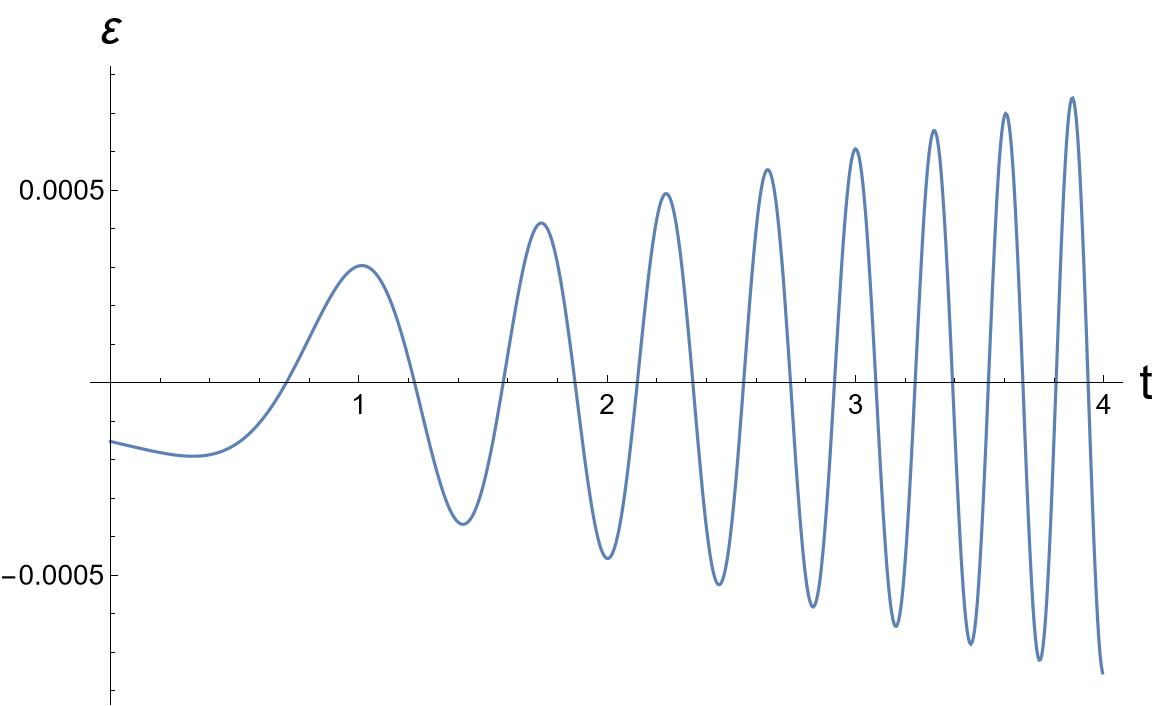
\includegraphics[width=0.65\textwidth]{T2_1}
	  	\caption{Зависимость полных деформаций от времени}
	  	\label{fig:p4}
	  \end{figure}
	  
	  \begin{figure}[H]
	  	\centering
	  	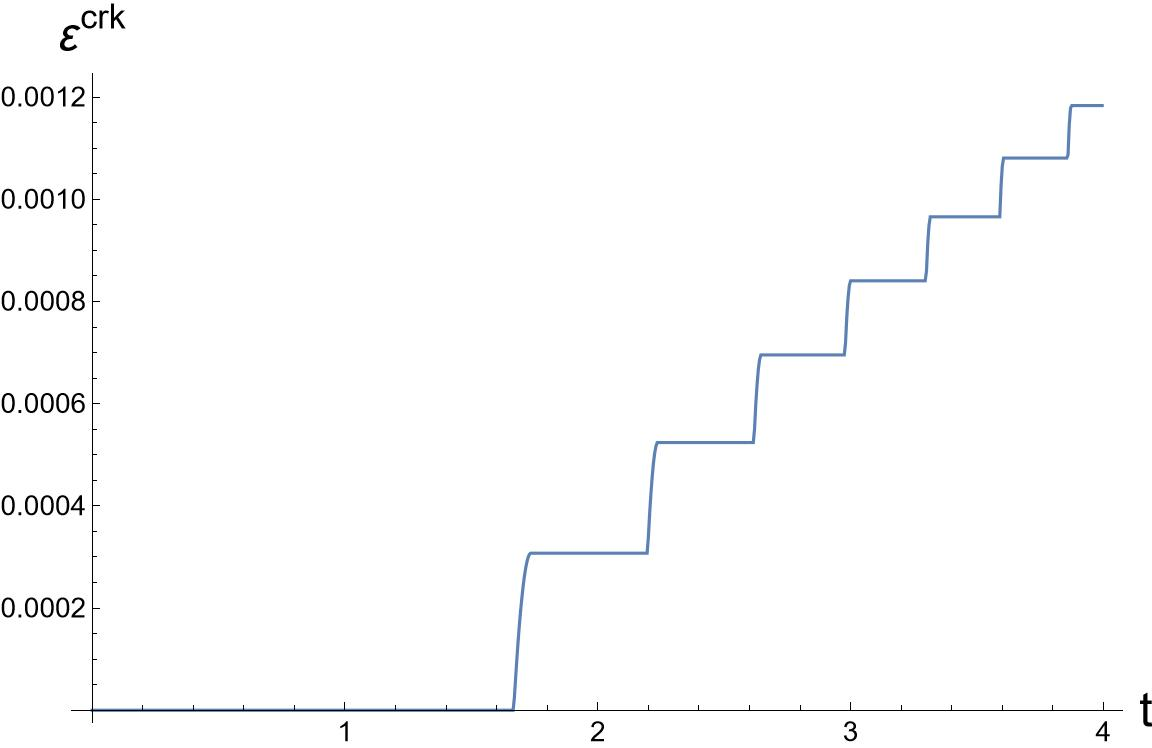
\includegraphics[width=0.65\textwidth]{T2_2}
	  	\caption{Зависимость деформаций за счет трещин от времени}
	  	\label{fig:p5}
	  \end{figure}
	  	  
	  \begin{figure}[H]
	  	\centering
	  	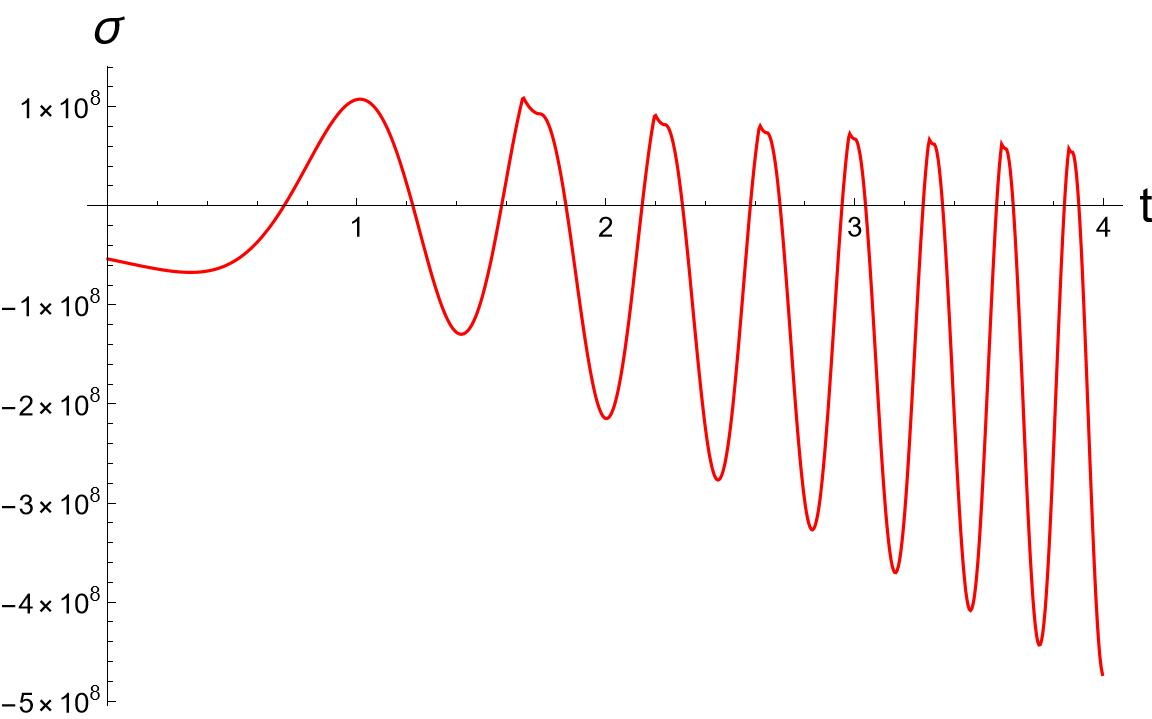
\includegraphics[width=0.65\textwidth]{T2_3}
	  	\caption{Зависимость напряжений от времени}
	  	\label{fig:6}
	  \end{figure}
	  
	  \begin{figure}[H]
	  	\centering
	  	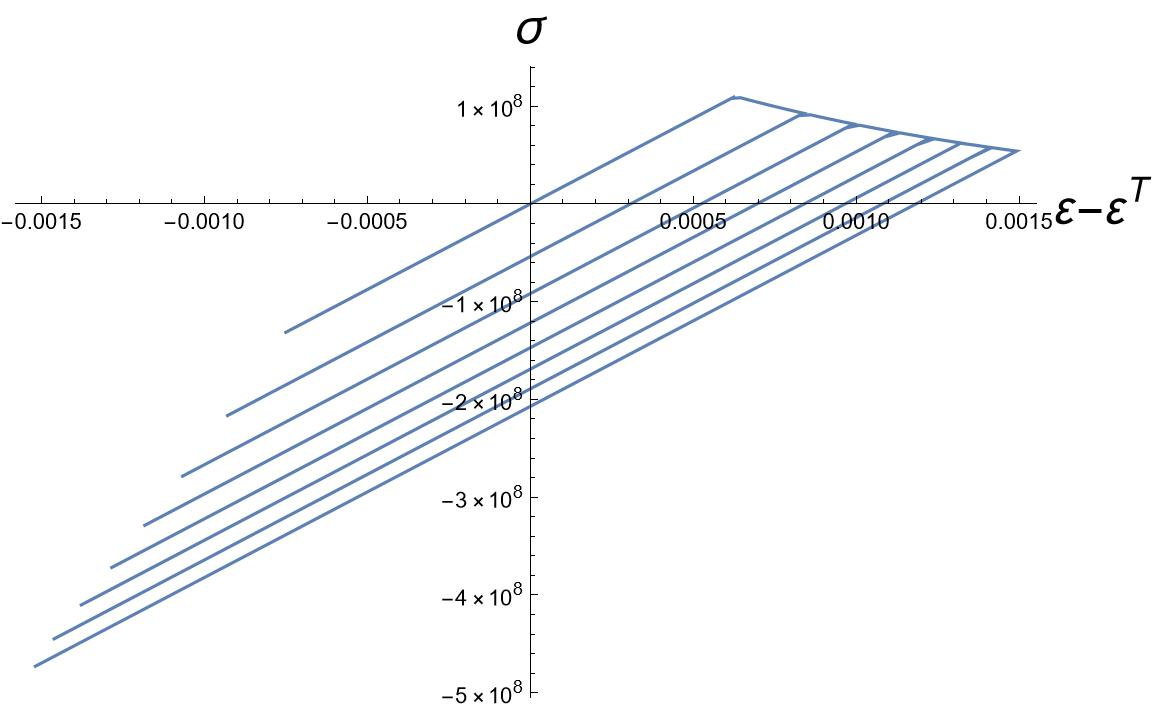
\includegraphics[width=0.6\textwidth]{T2_4}
	  	\caption{Зависимость напряжений от деформаций}
	  	\label{fig:p7}
	  \end{figure}
	  
	  \begin{figure}[H]
	  	\centering
	  	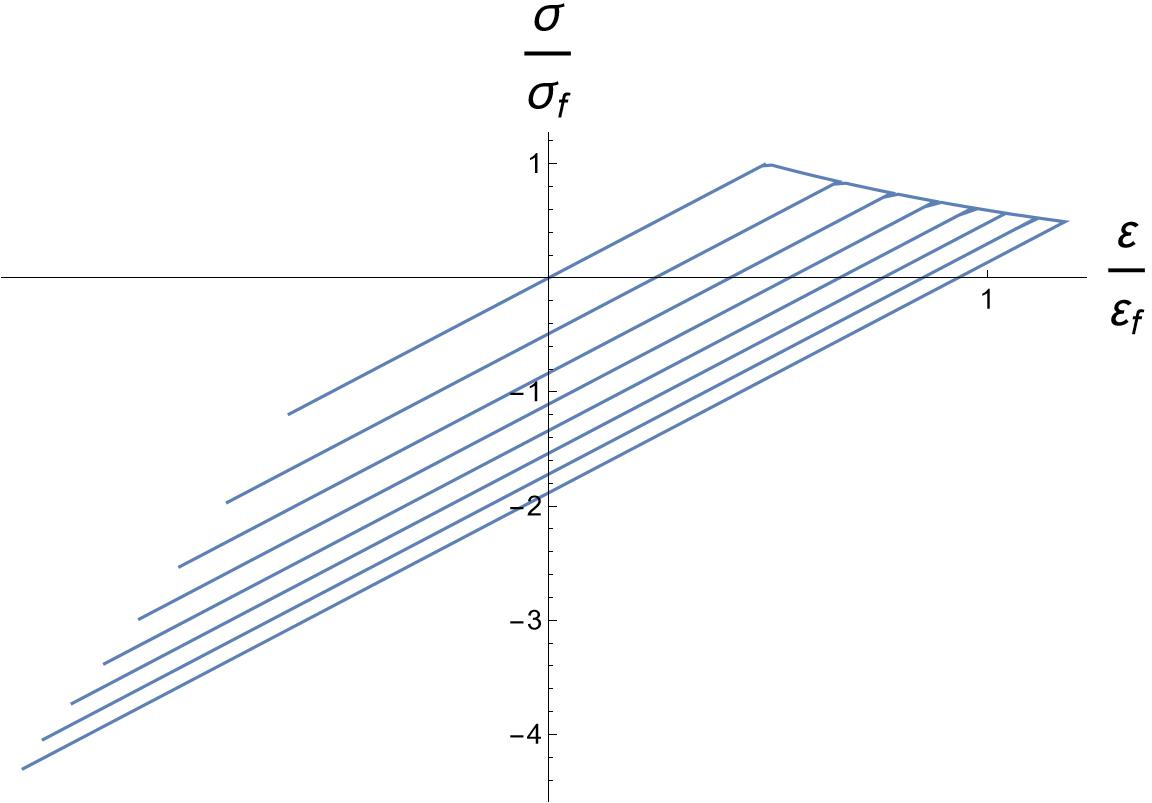
\includegraphics[width=0.6\textwidth]{T2_5}
	  	\caption{Зависимость напряжений от деформаций по отношению к пределам прочности}
	  		\label{fig:p8}
	  \end{figure}
	  
	  \begin{figure}[H]
	  	\centering
	  	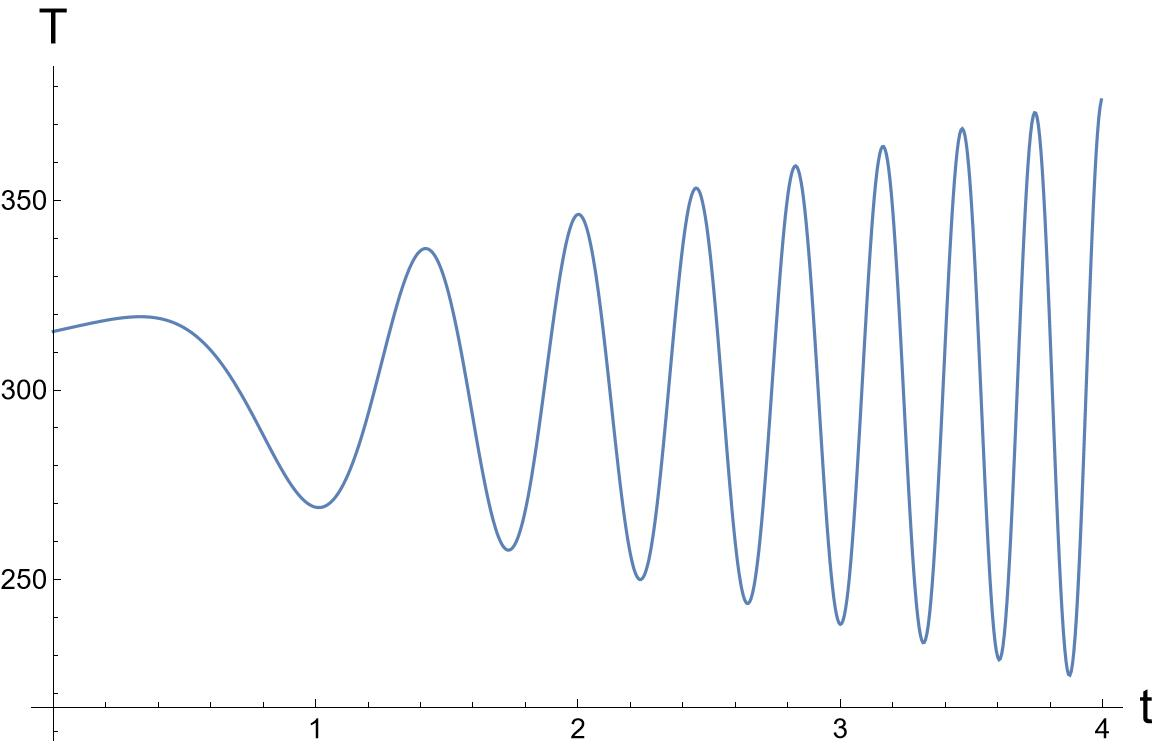
\includegraphics[width=0.6\textwidth]{T2_6}
	  	\caption{Зависимость температуры от времени}
	  		\label{fig:p9}
	  \end{figure}
  
  Периодическая зависимость полной деформации от времени приведена на рис.~\ref{fig:p4}.
  На рис.~\ref{fig:p7} видно, что при значениях
  напряжений, больших предела прочности, происходит разгрузка материала
  по нелинейному убывающему закону, в свою очередь, при уменьшении $\varepsilon-\varepsilon^T$ разгрузка по линейному закону с модулем Юнга, равным исходному. После этого происходит повторный этап нагружения по той же прямой, по которой происходила разгрузка, и далее цикл нагружения и разгрузки повторяется.
  
  На рис.~\ref{fig:p5} график имеет ступенчатый вид, что подтверждает цикличность процесса «нагрузка-разгрузка», а также способность модели накапливать информацию о разрушении стержня в предыдущие моменты времени.
  
Также, на рис.~\ref{fig:p8} можно увидеть, что в области $\sigma>0$ график ограничен экспериментальной кривой, которая показана на рис.~\ref{fig:ceramic}.

  	\item Пусть $\quad F(x) = a \sin\left(\sfrac{\pi x}{l}\right),\quad \tau(t) = t\sin(t),\quad a = 50,\quad T_f = 20 \text{ c}.$
  
  Аналитическое решение:
  %	\[
  %	\frac{\pl^2 u }{\pl x^2}=\alpha\frac{\pl}{\pl x}\left(\tilde T+a\sin\left(\frac{\pi x}{l}\right)t\sin(t)\right)\quad \Rightarrow \quad
  %	u = \alpha\frac{ a t \sin(t)}{\pi}\left(l-2x-l\cos\left(\frac{\pi x}{l}\right)\right)
  %	\]
  %\[
  %\frac{\pl^2 u }{\pl x^2}=\alpha\frac{\pl}{\pl x}\left(\tilde T+a\sin\left(\frac{\pi x}{l}\right)t\sin(t)\right)\]
  \[
  u(x, t) = \alpha\frac{ a t \sin(t)}{\pi}\left(l-2x-l\cos\left(\frac{\pi x}{l}\right)\right).
  \]
  
  \begin{figure}[H]
  	\centering
  	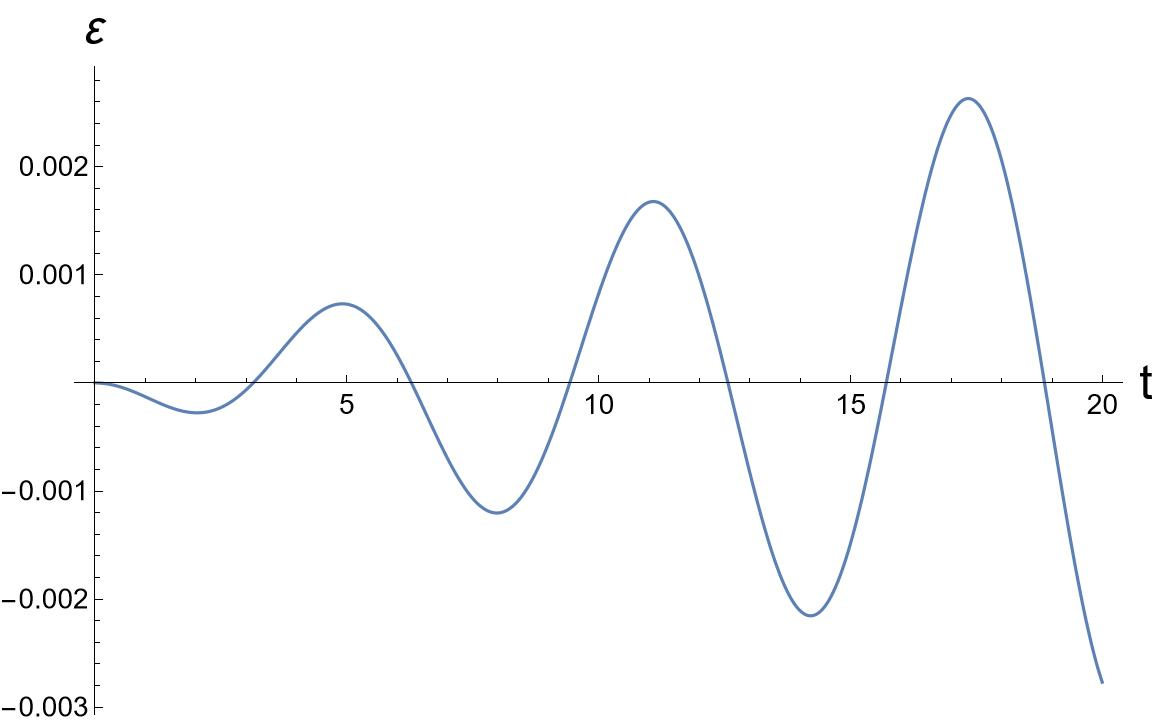
\includegraphics[width=0.49\textwidth]{T1_1}
  	\caption{Зависимость полных деформаций от времени}
  \end{figure}
  
  \begin{figure}[H]
  	\centering
  	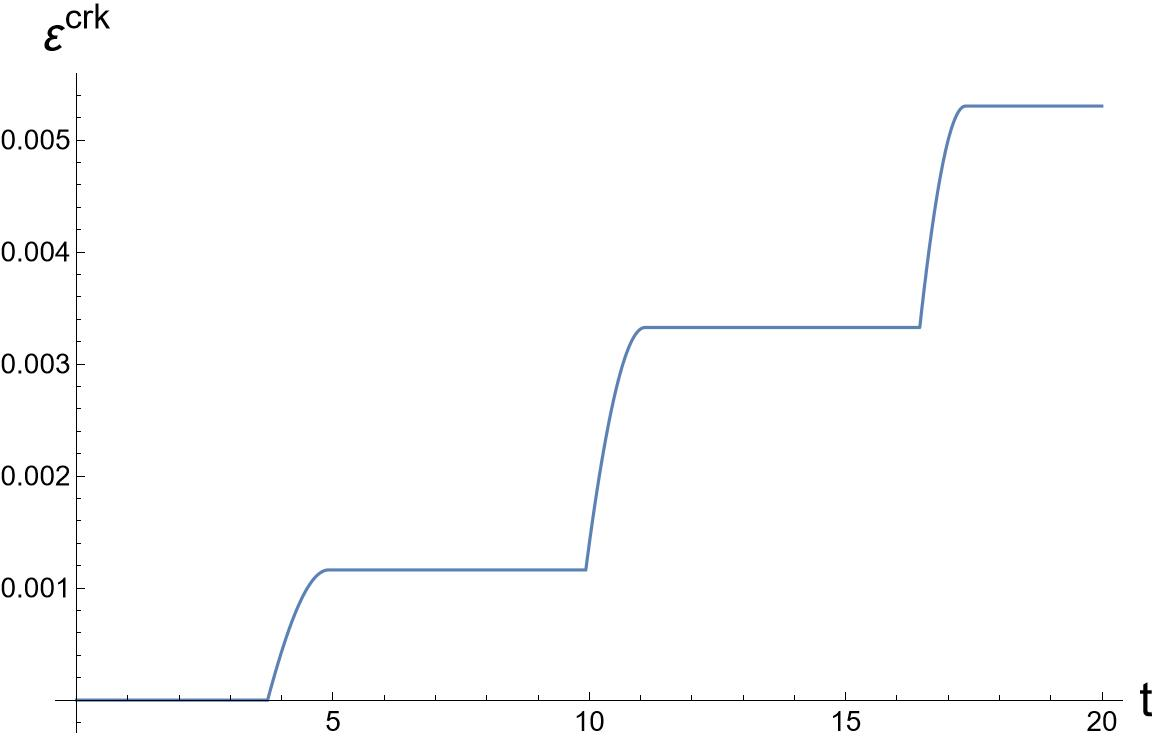
\includegraphics[width=0.63\textwidth]{T1_2}
  	\caption{Зависимость деформаций за счет трещин от времени}
  \end{figure}
  
  \begin{figure}[H]
  	\centering
  	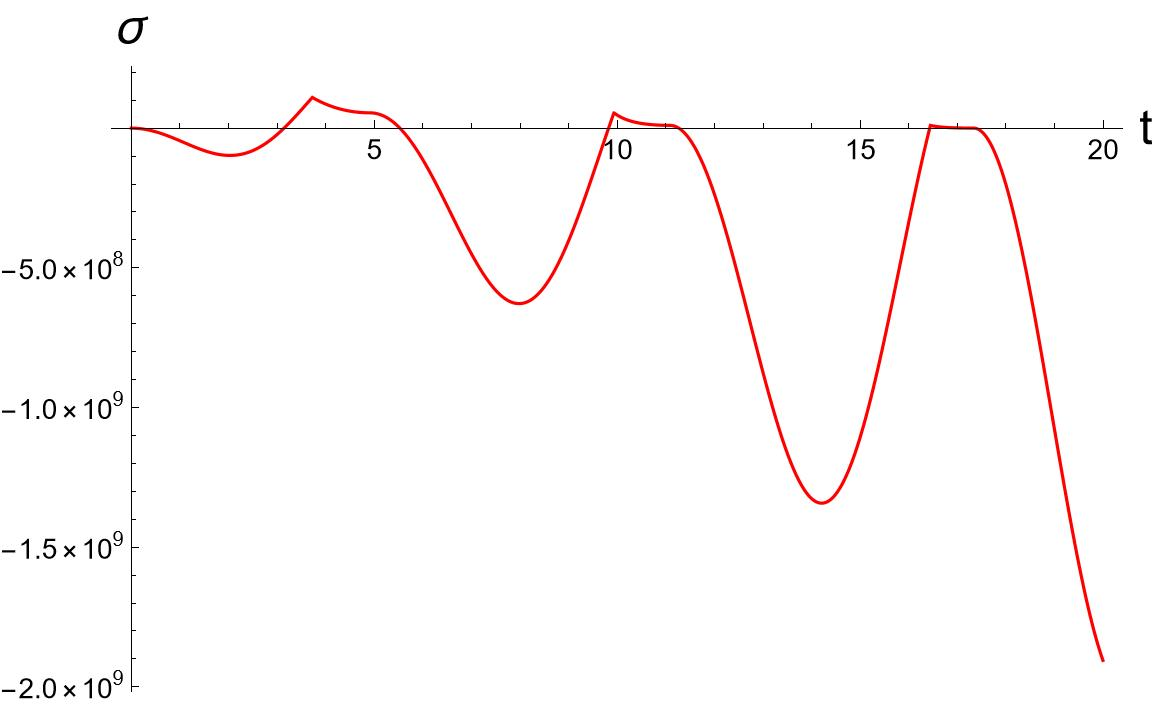
\includegraphics[width=0.63\textwidth]{T1_3}
  	\caption{Зависимость напряжений от времени}
  \end{figure}
  
  \begin{figure}[H]
  	\centering
  	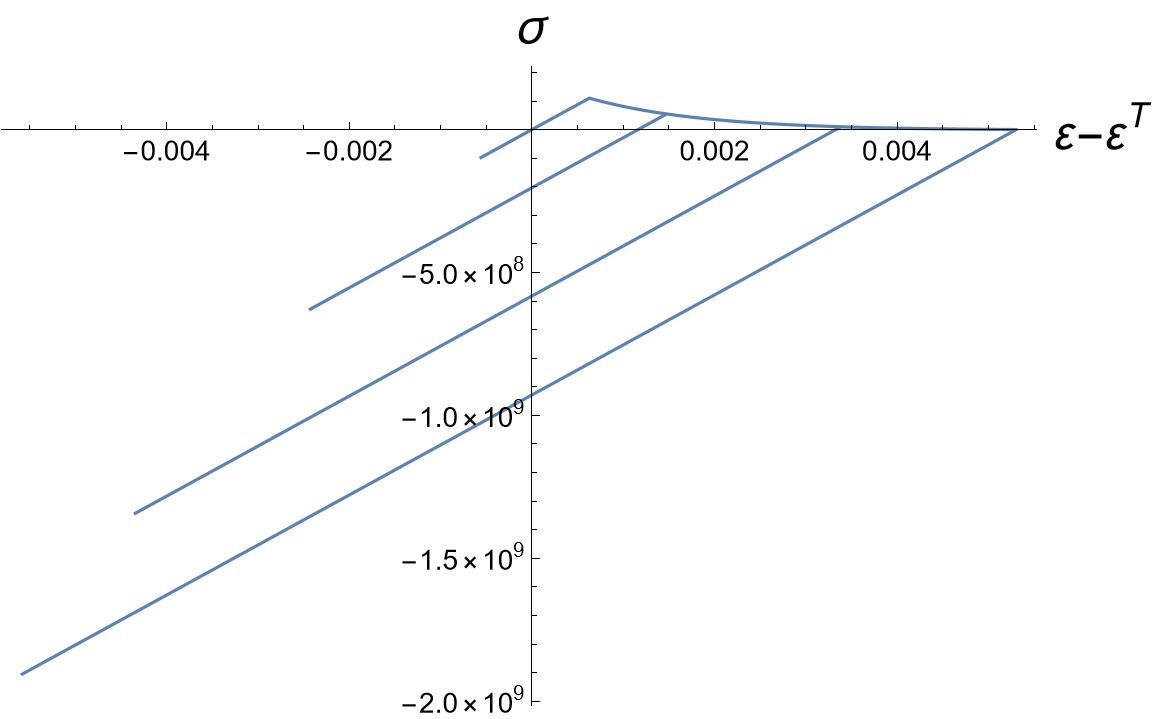
\includegraphics[width=0.63\textwidth]{T1_4}
  	\caption{Зависимость напряжений от деформаций}
  \end{figure}

  \begin{figure}[H]
  	\centering
  	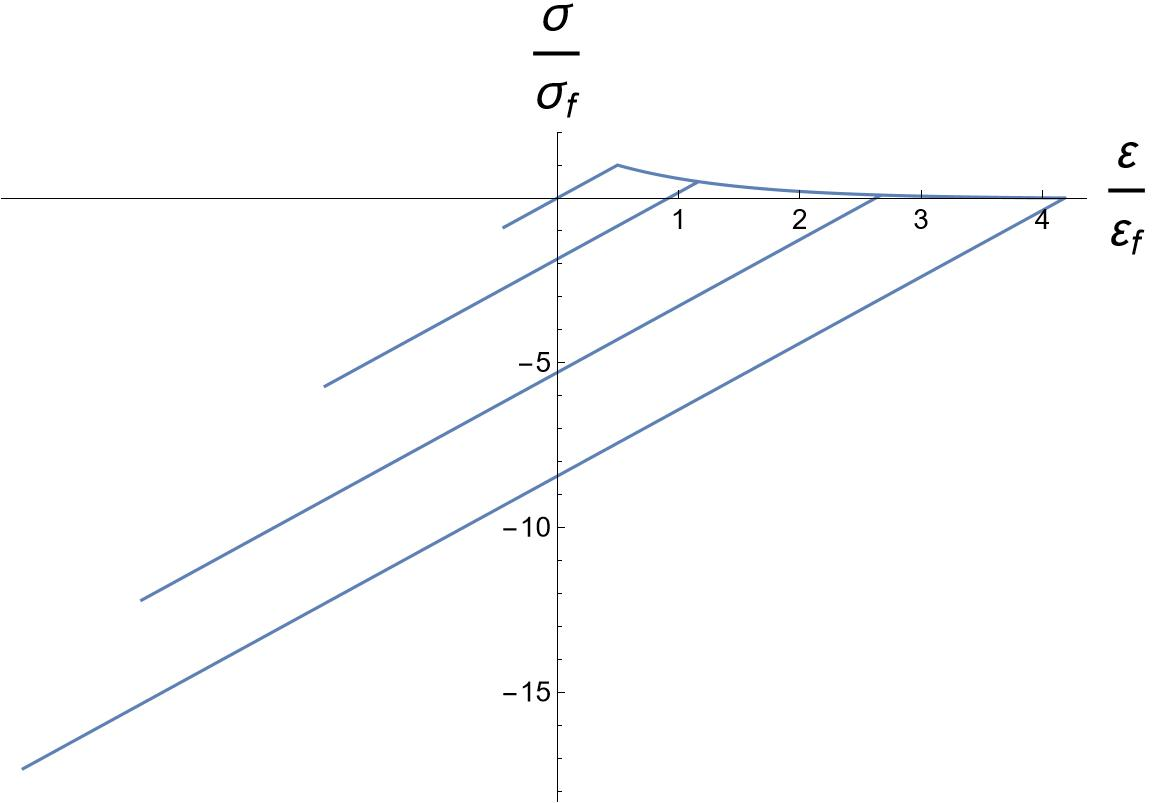
\includegraphics[width=0.63\textwidth]{T1_5}
  	\caption{Зависимость напряжений от деформаций по отношению к пределам прочности}
  \end{figure}
  
  \begin{figure}[H]
  	\centering
  	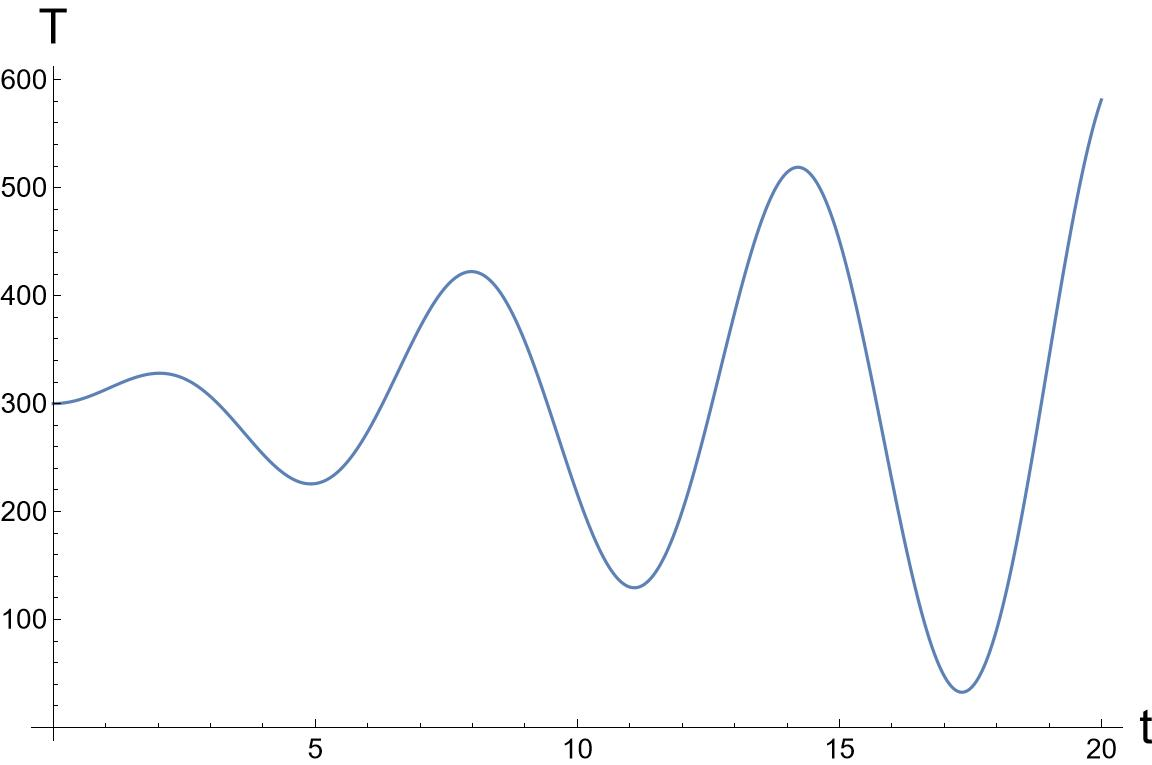
\includegraphics[width=0.63\textwidth]{T1_6}
  	\caption{Зависимость температуры от времени}
  \end{figure}
\end{enumerate}


	\section-{Заключение}
	В настоящей работе рассмотрена задача термоупругости для одномерного случая.
	Была исследована математическая модель разрушения стержня, состоящего из диоксида урана UO$_2$ и было найдено аналитическое решение для линейного случая. Данная задача была решена методом конечных разностей на равномерной сетке. Также, проведен графический анализ распространения трещин, основанный на графиках напряжений, деформаций и температур.
	
	 Решение вышеуказанной задачи было реализовано в системе компьютерной алгебры Wolfram Mathematica.
	
	\pagebreak
	\begin{thebibliography}{1}
		\bibitem{galanin1} \textit{Галанин М.П., Савенков Е.Б.} Методы численного анализа математических\\ моделей. М.: Изд-во МГТУ им. Н.Э. Баумана,	2010. 592 с.
		\bibitem{galanin2} Математическое моделирование разрушения хрупкого материала под действием тепловых нагрузок / М.П. Галанин [и др.] // Препринты ИПМ им. М.В. Келдыша. 2013. № 100. 36 с. URL:
		http://library.keldysh.ru/preprint.asp?id=2013-100.
		\bibitem{frost} \textit{Фрост Б.} ТВЭЛы ядерных реакторов: пер. с англ. М.: Энергоатомиздат, 1986. --
		\mbox{248 с.}
		\bibitem{zarubin} \textit{Зарубин В.С., Кувыркин Г.Н.} Математические модели механики и электродинамики сплошной среды. -- М.: Изд-во МГТУ им. Н.Э. Баумана, 2008. -- 512 с.: ил. (Математическое моделирование в технике и в технологии).
		\bibitem{timoshenko} \textit{Тимошенко С.П., Гудьер Дж.} Теория упругости. М.: Наука, 1975. 576 с.
		\bibitem{kovalenko} \textit{Коваленко А.Д.} Основы термоупругости : учебное пособие / А.Д. Коваленко. -- Киев: Наукова думка, 1970. -- 307 с.
		\bibitem{smeared crack} \textit{ Dahlblom O., Ottosen N.S.} Smeared Crack Analysis of Concrete Using a	Nonlinear Fracture Model // Fracture Mechanics of Concrete. Nordiс Seminar Held at Division of Building Materials, November 6, 1986, p. 31-46.
		
		
	\end{thebibliography}
	
	
\end{document}
